%----------------------------------------------------------------------------------------
%	Methodology
%----------------------------------------------------------------------------------------

\chapter{Methodology} \label{Chapter 3}

\section{Tensorflow Lite Micro}

TensorFlow Lite Micro (TFLM)~\cite{tflm} is a version of TensorFlow Lite designed for microcontrollers and other embedded systems with limited memory and processing power. TFLM provides a lightweight inference engine optimized for running deep learning models on devices with constrained resources. It supports a wide range of hardware platforms and allows for easy deployment of models on microcontrollers. For example, it doesn't require any support for dynamic memory and doesn't expect to run under the operating system. It has a simple yet effective way of managing allocations in the static memory of the program, using a two-stack allocation strategy and bin packing.% illustrated in Figure~\ref{fig:tflm_alloc}. 

TFLM has several useful features that make it a popular choice for AI model deployment on microcontrollers. For example, it supports a variety of neural network architectures, including convolutional, recurrent, and fully connected networks. It also includes a range of pre-trained models that can be used for various tasks, such as image classification and voice recognition. Additionally, TFLM provides tools for quantization, which is a process that allows models to be compressed and run more efficiently on resource-constrained devices.

However, TFLM also has some limitations that should be considered when using it for AI model deployment. One limitation is that it only supports a limited subset of TensorFlow operations, which means that some models may not be fully compatible with TFLM. Additionally, TFLM doesn't support training, only inference.

% \begin{figure}[t]
% \centering
% \caption{Two-stack allocation strategy~\cite{tflm}}
% 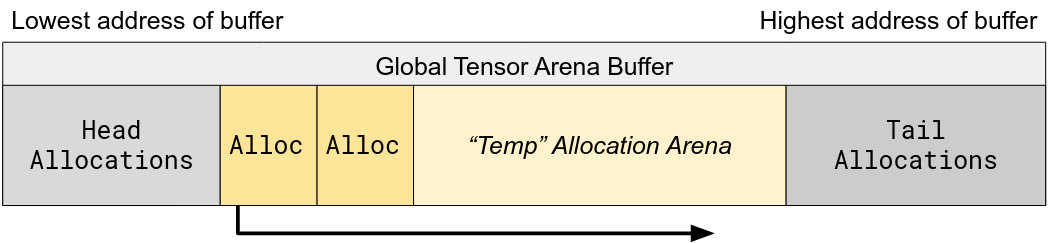
\includegraphics[width=1\textwidth]{tflm_allocation.png}
% \label{fig:tflm_alloc}
% \end{figure}

\section{CFU-Playground}\

To develop a custom Function Unit (CFU) for accelerating AI workloads, we will use the CFU-Playground tool described in~\cite{cfu_playground}. CFU-Playground is an open-source framework that provides a platform for developing and testing custom CFUs for RISC-V processors. The framework includes tools and scripts to create Custom Function Unit for a RISC-V soft-core. It can test performance and profile design, run a simulation of the processor, and synthesize it to deploy on the FPGA board. CFU-Playground supports different tools to conduct place and route and generate FPGA bitstream. It is integrated with TensorFlow lite micro (TFLM) for deployed ML model interference. 

The main idea is to find hotspots -- places in the model code where most CPU time is spent. Usually, such hotspots include repeated simple operations, such as multiply-add accumulate and matrix multiplications. Some code may require logical operations, such as quantizing calculated results. These kinds of operations can be implemented very efficiently in the hardware and map perfectly to the parallel nature of FPGA. 

\subsection{Soft core}

VexRiscV~\cite{vexriscv} is a soft processor implementation of the RISC-V ISA that is open-source and fully customizable. It implements RV32I base integer instruction set and with a subset of standard extensions\footnote{[M][A][F[D]][C]: ''M'' -- Integer Multiplication and Division, ''A'' -- Atomic Instructions, ''F/D'' -- Single/Double Point Precision Point, ''C'' -- Compressed instructions~\cite{risc_v_manual}.} ISA and pipeline from 2 to 5+ stages ([Fetch*X], Decode, Execute, [Memory], [WriteBack]). Its small and efficient design makes it ideal for embedded systems with limited resources. Additionally, VexRiscV has built-in support for various extensions, including custom instructions and support for plugins. 

VexRiscV was chosen as the platform for developing the custom CFU in CFU-Playground. VexRiscV is one of the few soft processors that support the CFU extension. Also, it is synthesizable on the FPGA and doesn't require many resources, which leaves more FPGA resources to be allocated for the custom CFU. It is very flexible. A developer can change a number of caches, cache sizes, and pipeline stages and add custom instructions. 

\subsection{HDL}

Hardware Description Language (HDL) is a specialized computer language that describes the behavior of digital circuits and systems. HDLs can be used to create high-level behavioral models of digital circuits or low-level designs that specify individual logic gates and connections. Verilog and its successor SystemVerilog are a popular HDL for designing digital systems. They are commonly used to design digital circuits, such as CPUs, FPGAs, and ASICs. Verilog has a C-like syntax, providing features such as modules, functions, and procedural constructs to describe digital circuits. Verilog and SystemVerilog are standardized by the Institute of Electrical and Electronics Engineers under the standards of IEEE 1364-2005~\cite{verilog_standard} and IEEE 1800-2017~\cite{system_verilog_standard}, respectively.

\subsection{Simulation}

Simulating hardware design is an important step in developing any hardware system. CFU-Playground uses Renode~\cite{renode} to simulate the processor and CFU together. Renode is a framework developed by Antmicro for simulating IoT devices. It can simulate heterogeneous multicore SoCs and various peripherals. The processor is simulated on the ISA level. Renode supports the most popular ISAs, like ARMv7 and ARMv8, X86, RISC-V, SPARC, POWER, and Xtensa. CFU is simulated in a cycle-accurate Verilator simulation. 

\subsection{Synthesis. Place and Route}

Synthesis translates the hardware design, described in a Hardware Description Language (HDL) such as Verilog, into a netlist that describes the logical functions and their interconnections. The synthesis tool considers the constraints of the target device and the timing requirements of the design. The output of the synthesis tool is a gate-level netlist, which represents the hardware design in terms of primitive logic gates. CFU-Playground supports open source Yosys~\cite{yosys} and Vivado synthesis tool~\cite{vivado_synthesis} for Xilinx FPGA boards for the design synthesis. 

Place and Route is the process of determining the physical placement of the logic elements in the FPGA and the routing of the interconnects between them. The place and route tool takes into account the physical constraints of the target device, such as the number of available logic elements, the number of I/O pins, and the routing resources. The output of the place and route tool is a bitstream file that can be loaded onto the FPGA to program the device. Vivado place and route tool~\cite{vivado_implementation} does this for Xilinx FPGA boards. An open-source alternative is Verilog to Routing's~\cite{vtr8} tool called ''Versatile Place and Route'' (vpr) combined with an f4pga~\cite{f4pga} bitstream generator. 